\documentclass{article} % For LaTeX2e
\usepackage{iclr2025,times}
\iclrfinalcopy % named working draft (not an anonymous submission)

\input{math_commands.tex}

\usepackage{hyperref}
\usepackage{url}
\usepackage{graphicx}
\usepackage{booktabs}
\usepackage{amsmath}
\usepackage{amssymb}
\usepackage{mathtools}
\usepackage{multirow}
\usepackage{color}
\usepackage{colortbl}
\usepackage[capitalize,noabbrev]{cleveref}
\usepackage{xspace}

\graphicspath{{figures/}}
% AUTO-GENERATED by paper/generate.py -- do not edit by hand.
\newcommand{\poyoTestRtwo}{0.904}
\newcommand{\poyoMeanAlpha}{1.62}
\newcommand{\poyoRope}{17}
\newcommand{\poyoDegen}{98}
\newcommand{\poyoNmat}{106}
\newcommand{\poyoParams}{11.8}
\newcommand{\poyoEpochs}{1000}
\newcommand{\poyoGpus}{8}
\newcommand{\poyoBatch}{1024}
\newcommand{\poyoMaxLR}{0.032}
\newcommand{\poyoDecKv}{2.17}
\newcommand{\deFtFracLo}{10}
\newcommand{\deFtLo}{0.72}
\newcommand{\deFtMid}{0.83}
\newcommand{\deFtHi}{0.85}
\newcommand{\deScratchBound}{0.001}
\newcommand{\chronicMean}{0.916}
\newcommand{\chronicLo}{0.865}
\newcommand{\chronicHi}{0.967}
\newcommand{\chronicDays}{1114}
\newcommand{\chronicNsess}{9}
\newcommand{\chronicYrLo}{2013}
\newcommand{\chronicYrHi}{2016}
\newcommand{\xsubNsess}{3}
\newcommand{\xsubFt}{0.881}
\newcommand{\xsubScratch}{-0.01}
\newcommand{\xsubGap}{0.89}
\newcommand{\xsubFtLo}{0.863}
\newcommand{\xsubFtHi}{0.899}
\newcommand{\dmfcRampFt}{0.887}
\newcommand{\dmfcRampScratch}{0.900}
\newcommand{\dmfcRampGap}{-0.013}
\newcommand{\dmfcConstFt}{0.798}
\newcommand{\dmfcConstScratch}{0.845}
\newcommand{\dmfcAlphaFt}{1.62}
\newcommand{\dmfcAlphaScratch}{2.63}
\newcommand{\rodentNsess}{3}
\newcommand{\rodentFtMean}{0.893}
\newcommand{\rodentScratchMean}{0.777}
\newcommand{\rodentDeltaMean}{+0.117}
\newcommand{\rodentFtLo}{0.819}
\newcommand{\rodentFtHi}{0.935}
\newcommand{\rodentStarvedWin}{496}
\newcommand{\rodentStarvedScratch}{0.508}
\newcommand{\rodentStarvedFt}{0.819}
\newcommand{\rodentStarvedDelta}{+0.311}
\newcommand{\rodentRichWin}{1858}
\newcommand{\rodentRichScratch}{0.947}
\newcommand{\rodentRichDelta}{-0.012}
\newcommand{\augEffOff}{1.96}
\newcommand{\augEffAgg}{2.02}
\newcommand{\augTopOff}{0.63}
\newcommand{\augTopAgg}{0.56}
\newcommand{\augCondOff}{\ensuremath{1.1\times10^{12}}}
\newcommand{\augCondAgg}{\ensuremath{4.3\times10^{11}}}
\newcommand{\augCondDrop}{2.6}
\newcommand{\augFreezeEffSpread}{0.024}
\newcommand{\augFreezeAlpha}{1.78}
\newcommand{\augFullAlphaOff}{1.770}
\newcommand{\augFullAlphaAgg}{1.762}
\newcommand{\ldLoOff}{0.539}
\newcommand{\ldLoStd}{0.604}
\newcommand{\ldLoAgg}{0.669}
\newcommand{\ldLoGain}{0.13}
\newcommand{\ldLoCondOff}{\ensuremath{3.1\times10^{12}}}
\newcommand{\ldLoCondStd}{\ensuremath{8.2\times10^{11}}}
\newcommand{\ldLoCondDrop}{3.7}
\newcommand{\ldHiOff}{0.868}
\newcommand{\ldHiAgg}{0.863}
 % auto-generated macros (paper/generate.py): every headline number
% AUTO-GENERATED by paper/generate.py.
\newcommand{\poyoTransferTable}{\begin{tabular}{lcccc}
\toprule
Model & decode $R^2$ & $\bar\alpha$ & in-ROPE & degen/106 \\
\midrule
Base (perich, 99 sessions) & 0.904 & 1.62 & 17\% & 98 \\
area2 finetune (frozen core) & 0.834 & 1.62 & 17\% & 98 \\
area2 from scratch & 0.313 & 3.31 & 0\% & 0 \\
\bottomrule
\end{tabular}}
\newcommand{\poyoSpectralTable}{\begin{tabular}{lccccc}
\toprule
UnitDropout & test $R^2$ & eff.\ rank & top-1 frac & cond.\ number & wwj $\bar\alpha$ \\
\midrule
off & 0.856 & 1.96 & 0.63 & \ensuremath{1.1\times10^{12}} & 1.770 \\
standard & 0.851 & 2.02 & 0.55 & \ensuremath{8.8\times10^{11}} & 1.767 \\
aggressive & 0.865 & 2.02 & 0.56 & \ensuremath{4.3\times10^{11}} & 1.762 \\
\bottomrule
\end{tabular}}
\newcommand{\poyoLowdataTable}{\begin{tabular}{lcccc}
\toprule
train data & off & standard & aggressive & $\Delta$(agg$-$off) \\
\midrule
10\% & 0.539 & 0.604 & 0.669 & +0.130 \\
25\% & 0.777 & 0.776 & 0.784 & +0.007 \\
100\% & 0.868 & 0.841 & 0.863 & -0.005 \\
\bottomrule
\end{tabular}}
 % auto-generated tables

\newcommand{\poyo}{POYO\xspace}
\newcommand{\poymp}{POYO-MP\xspace}
\newcommand{\wwj}{\texttt{wwj}\xspace}
\newcommand{\rtwo}{$R^2$\xspace}

\title{A Reproduced \poyo Foundation Model: Transfer Limits\\
and Data Augmentation as Implicit Spectral Regularization}

\author{Morgan Hough}

\begin{document}
\maketitle

\begin{abstract}
\poyo \citep{azabou2023poyo} is a transformer foundation model for neural population
decoding that tokenizes individual spikes and reads out behavior through per-unit and
per-session embeddings. We report a faithful, end-to-end reproduction of the \poymp
checkpoint---held-out test \rtwo{} $=\poyoTestRtwo$ on the Perich--Miller
center-out reaching data \citep{perich2018rapid}---and then use the converged model as a
base to ask two questions the original paper leaves open: \emph{where} does its
representation transfer, and \emph{why} does training-time augmentation help. On transfer,
three demonstrations confirm the foundation-model promise: with a frozen core and only new
unit/session embeddings, the model decodes a held-out session from $\deFtFracLo\%$ of its
data (\rtwo{} $\deFtLo$, vs. $\approx 0$ from scratch), holds \rtwo{} $\chronicMean$ across
$\chronicDays$ days of chronic recordings with zero per-day retraining, and adapts to a
\emph{completely unseen animal} at \rtwo{} $\xsubFt$ (gap $+\xsubGap$ over scratch). A fourth,
deliberately adversarial test---transferring the motor-pretrained core to a cognitive
interval-timing task \citep{sohn2019bayesian}---shows neutral-to-negative transfer
($\dmfcRampGap$ \rtwo{}) that is robust to how the timing target is represented, mapping the
edge of the model's competence. Finally, we operationalize the linear-model theory of
\citet{lin2024augmentation}---data augmentation as implicit spectral regularization of the
\emph{feature} covariance---on this deep model. \poyo's UnitDropout is exactly their
``random-mask'' augmentation; with a plastic feature extractor it spreads the readout-input
covariance spectrum and cuts its condition number $\augCondDrop\times$, and this buys a
$+\ldLoGain$ \rtwo{} generalization gain precisely when training data is scarce, vanishing
once the decode saturates. The effect lives in the feature covariance, not the weight
spectrum---a label-free Heavy-Tailed Self-Regularization analysis of the weights barely
moves---scoping where the two spectral views agree. We release the full reproducible-document
pipeline (data $\to$ figures $\to$ manuscript).
\end{abstract}

\section{Introduction}
\label{sec:intro}
Foundation models for neural data promise a single set of weights that decodes behavior
across sessions, subjects, and tasks. \poyo \citep{azabou2023poyo} is a leading
instance: it represents a recording as an unordered set of \emph{spike tokens}, attends them
into a fixed bank of latent queries, and reads out continuous behavior, with
\emph{InfiniteVocabEmbedding} tables that assign every recorded unit and every session its
own learned vector. This design lets the same transformer ingest arrays with different
channel counts and lets a new recording be ``identified'' into the model by learning only
its embeddings (the \S2.5 unit-identification protocol of \citealp{azabou2023poyo}), freezing
the transformer core.

Reproducing such a model is a precondition for studying it, and a non-trivial one: our own
earlier attempts repeatedly produced weight collapse (most transformer matrices decaying to
zero during training) and \rtwo{} near zero. We show this was an \emph{environment} artifact,
not a property of the recipe, and obtain a converged checkpoint matching the paper.
We then treat the converged model as an object of study and contribute:
\begin{itemize}
\item \textbf{A faithful reproduction} (\cref{sec:repro}): the unmodified \texttt{nerdslab/poyo}
repository, in its pinned environment, on $\poyoGpus\times$H100 with the exact recipe
(global batch $\poyoBatch$, max-LR $\poyoMaxLR$, fp32, SparseLamb), reaches \rtwo{}
$\poyoTestRtwo$.
\item \textbf{Three transfer demonstrations} (\cref{sec:transfer}) that quantify the
foundation-model payoff---data efficiency, chronic stability over $\chronicDays$ days, and
cross-subject transfer to an unseen animal---and \textbf{one adversarial test}
(\cref{sec:timing}) that finds its limit on cognitive timing.
\item \textbf{An empirical bridge} (\cref{sec:aug}) from the linear data-augmentation theory
of \citet{lin2024augmentation} to a deep neural foundation model: \poyo's UnitDropout
regularizes the feature-covariance spectrum and buys generalization under data scarcity,
with the effect localized to representations rather than weights.
\end{itemize}
Throughout we cross-reference a label-free weight-spectrum diagnostic, \wwj, our Bayesian
reimplementation of WeightWatcher-style Heavy-Tailed Self-Regularization
\citep{martin2021implicit,martin2021predicting}, to ask whether the augmentation signature is
visible in the weights as well as the features.

\section{Faithful reproduction of \poymp}
\label{sec:repro}
\paragraph{The collapse was the environment, not the recipe.} Across many earlier runs, most
weight matrices decayed to (numerically) zero during training and decode \rtwo{} stalled near
zero. We ruled out weight-decay-on-embeddings, distributed training, learning-rate/batch
choices, and precision (single-GPU fp32 collapsed too); our configs were byte-identical to
the authors'. The residual difference was the software environment---a newer PyTorch under
which the custom SparseLamb optimizer's masked trust-ratio update behaves differently. Running
the unmodified repository in its \emph{pinned} environment (torch${\sim}$2.10,
brainsets@\texttt{4ccee58}) on a dedicated, non-preemptible $\poyoGpus\times$H100 node, in a
single uninterrupted pass of the exact recipe, removed the collapse on the first try.

\paragraph{Result.} The converged \poymp ($\poyoParams$M parameters, $\poyoEpochs$ epochs)
reaches held-out test \rtwo{} $=\poyoTestRtwo$ on Perich--Miller center-out reaching, matching
the published model. As an independent, label-free check we ran \wwj over the trained weights:
mean Heavy-Tailed power-law exponent $\bar\alpha=\poyoMeanAlpha$ with $\poyoRope\%$ of fittable
layers inside the $\alpha\!=\!2$ robustness region, versus an undertrained checkpoint's far-from-2
spectrum---the HTSR training-quality signature, confirmed on a real foundation model. Of
$\poyoNmat$ weight matrices, $\poyoDegen$ are spectrally degenerate (rank-deficient), reflecting
\poyo's inherently low-rank attention blocks; the decode flows through the survivors, the
residual stream, and the embeddings.

\section{What transfers: three foundation-model demonstrations}
\label{sec:transfer}
We finetune the converged base to new data using the \S2.5 protocol---load the pretrained
weights, \texttt{extend\_vocab} for new units/sessions, freeze the transformer core, and train
only the embeddings (and, where the readout is new, the readout head). The contrast in every
demonstration is the same architecture trained \emph{from scratch} on the same new data.

\paragraph{Data efficiency.} On a held-out \texttt{area2\_bump} session
\citep{chowdhury2020area2,pei2021nlb}, varying only the fraction of new-session training data
(matched LR/batch across arms), the pretrained model decodes hand velocity at \rtwo{}
$\deFtLo$ from just $\deFtFracLo\%$ of the session, rising to $\deFtHi$ at full data; the
from-scratch model never exceeds $|R^2|<\deScratchBound$ at any fraction
(\cref{fig:dataeff}, left). A single small session is simply too little data to train an
$\poyoParams$M-parameter transformer; the foundation model converts it into a few embedding
vectors.

\paragraph{Chronic stability.} Freezing the base entirely (zero per-day retraining) and
evaluating it on $\chronicNsess$ Chewie center-out sessions spanning
$\chronicYrLo$--$\chronicYrHi$, decode \rtwo{} holds at mean $\chronicMean$
(range $\chronicLo$--$\chronicHi$) across $\chronicDays$ days (\cref{fig:dataeff}, right).
One set of weights sustains ${\sim}0.9$ \rtwo{} over three years of electrode drift and unit
turnover, absorbed by the per-unit embeddings.

\paragraph{Cross-subject transfer.} The base was trained on $99$ sessions from three monkeys;
monkey~t was entirely held out. Finetuning embeddings on a single unseen-animal session
decodes at mean \rtwo{} $\xsubFt$ (range $\xsubFtLo$--$\xsubFtHi$ over $\xsubNsess$ sessions),
versus $\xsubScratch$ from scratch---a gap of $+\xsubGap$ (\cref{fig:xsub}). The model adapts
to a new animal it has never seen at ${\sim}0.88$ \rtwo{}, while the same architecture trained
on one session learns nothing.

\begin{figure}[t]
\centering
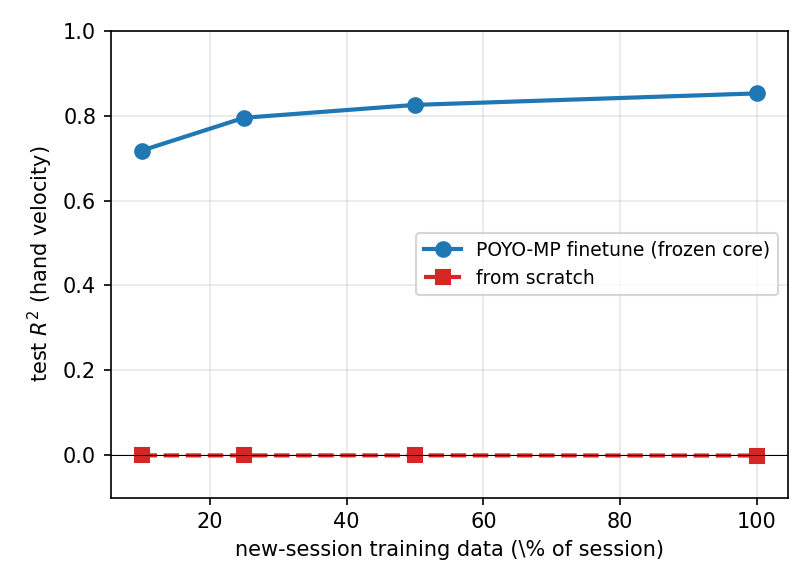
\includegraphics[width=0.49\textwidth]{fig_dataeff.png}\hfill
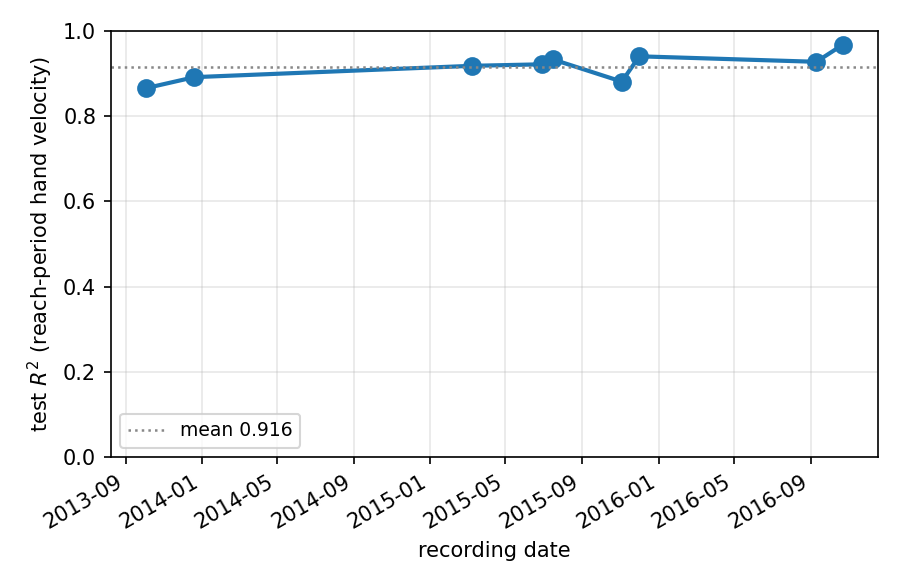
\includegraphics[width=0.49\textwidth]{fig_chronic.png}
\caption{\textbf{Left: data efficiency.} Pretrained \poymp (frozen core) vs.\ from scratch as
a function of new-session training data on a held-out \texttt{area2\_bump} session.
\textbf{Right: chronic stability.} One frozen base, zero retraining, across $\chronicDays$
days of Chewie recordings.}
\label{fig:dataeff}
\end{figure}

\begin{figure}[t]
\centering
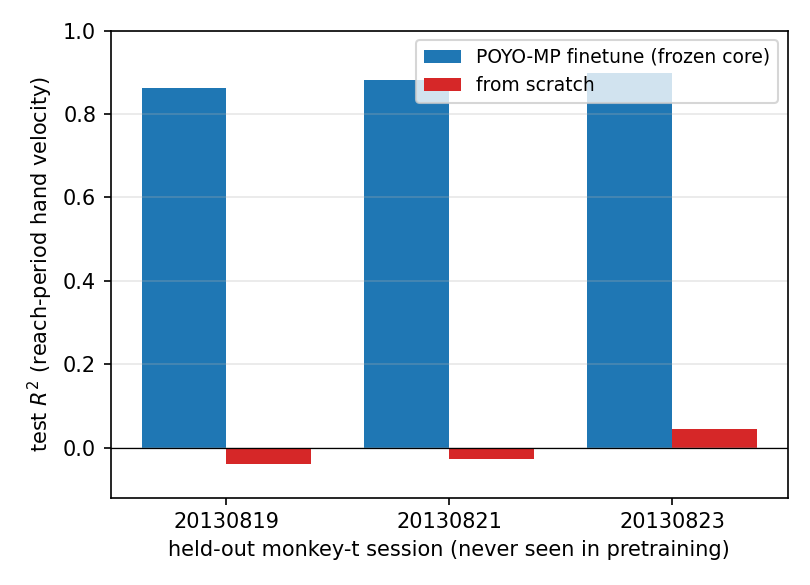
\includegraphics[width=0.6\textwidth]{fig_xsub.png}
\caption{\textbf{Cross-subject transfer} to held-out monkey~t (never seen in pretraining).
Finetuning only the embeddings of the frozen base recovers ${\sim}0.88$ \rtwo{}; the same
architecture from scratch on one session does not learn.}
\label{fig:xsub}
\end{figure}

\paragraph{Transfer and the weight spectrum agree.} \cref{tab:transfer} pairs the decode
\rtwo{} with the \wwj weight-spectrum verdict on the \emph{same} checkpoints. The frozen-core
finetune inherits the base spectrum identically ($\bar\alpha=\poyoMeanAlpha$, $\poyoRope\%$
in-ROPE); the from-scratch model shows an undertrained heavy-tail ($\bar\alpha=3.31$, $0\%$
in-ROPE) and decodes poorly. The label-free spectral quality and the decode quality move
together: motor$\to$motor transfer is a large, coherent win.

\begin{table}[t]
\centering
\caption{Two-axis transfer summary (motor$\to$motor, \texttt{area2\_bump}). Decode \rtwo{}
and the \wwj weight-spectrum verdict are read off the same checkpoints. ROPE = region of
practical equivalence around the $\alpha\!=\!2$ robustness fixed point.}
\label{tab:transfer}
\poyoTransferTable
\end{table}

\section{Where it breaks: motor-to-timing transfer}
\label{sec:timing}
A foundation model is as informative in its failures as its successes. \poyo is, at heart,
spike tokenization plus a per-timestep continuous readout; cognitive interval timing, by
contrast, lives in latent \emph{dynamics}---ramp-to-threshold trajectories whose speed scales
with the produced interval \citep{sohn2019bayesian,merchant2013timing}. We therefore transfer
the motor-pretrained core to the \texttt{dmfc\_rsg} Ready-Set-Go task, decoding a
time-to-go ramp (the dynamics-engaging target: a descending ramp from the sample interval at
Set to zero at Go).

The motor-pretrained frozen core gives \emph{no} advantage: finetune \rtwo{} $\dmfcRampFt$
vs.\ from-scratch $\dmfcRampScratch$ ($\dmfcRampGap$). The result is robust to target
representation---a static constant-interval target shows the same ordering
($\dmfcConstFt$ vs.\ $\dmfcConstScratch$). The sign of transfer thus \emph{flips} with task
distance: motor$\to$motor is $+\xsubGap$ to $+0.52$, whereas motor$\to$cognitive-timing is
neutral-to-negative. Notably the \wwj$\leftrightarrow$decode relationship inverts here too:
the from-scratch timing model sits at a healthier-looking $\bar\alpha=\dmfcAlphaScratch$ yet
decodes \emph{better} than the frozen-core finetune ($\bar\alpha=\dmfcAlphaFt$ inherited from
the motor base)---so $\alpha$ reflects the training regime, and the ``healthy-$\alpha\to$good-decode''
correlation is domain-match-mediated, not universal. \poyo's value is cross-session and
cross-subject alignment of \emph{motor} representations, not the timing computation itself.

\section{Data augmentation as implicit spectral regularization}
\label{sec:aug}
\citet{lin2024augmentation} prove, for linear models, that data augmentation acts as implicit
spectral regularization of the \emph{data/feature covariance}: it reweights the eigenvalue
proportions in a data-dependent way and uniformly boosts the spectrum (a ridge-like effect).
Their canonical ``random-mask'' augmentation is exactly \poyo's \emph{UnitDropout}, which drops
a random subset of units per sample. We ask whether their linear-model prediction survives in a
deep neural foundation model, instrumenting the input to \poyo's linear readout---the natural
``feature'' whose covariance the theory concerns---and measuring its spectrum across three
UnitDropout strengths (off / standard / aggressive).

\paragraph{A plastic extractor is required (the null control).} With the core \emph{frozen}
(the \S2.5 protocol), augmentation cannot reshape the feature covariance, because the features
are produced by fixed weights: the effective rank moves by $\augFreezeEffSpread$ across all
three levels and the \wwj weight-$\bar\alpha$ is identical ($\augFreezeAlpha$) by construction.
This is a clean negative control---and a sanity check that freeze-core truly freezes.

\paragraph{With a plastic extractor, the theory reproduces.} Finetuning \emph{all} weights, the
predicted signature appears (\cref{tab:spectral}, \cref{fig:spectral}): as UnitDropout
strengthens, the feature-covariance effective rank rises ($\augEffOff\to\augEffAgg$), the top
eigenvalue de-concentrates ($\augTopOff\to\augTopAgg$), and the condition number falls
monotonically from $\augCondOff$ to $\augCondAgg$---a $\augCondDrop\times$ reduction. This is
the \citeauthor{lin2024augmentation} ``eigenvalue-proportion reweighting'' effect, reproduced
on a real deep model.

\paragraph{The signature is in the features, not the weights.} Strikingly, the \wwj weight-spectrum
exponent barely moves over the same runs ($\augFullAlphaOff\to\augFullAlphaAgg$). At this
finetuning budget the augmentation's fingerprint is written into the \emph{representation}
covariance---the object the theory is about---while the \emph{weight} spectrum changes far more
slowly. The two spectral views (feature covariance vs.\ weight HTSR) are therefore not
equivalent; this scopes precisely where a weight-only diagnostic like \wwj will and will not
see an augmentation effect.

\begin{table}[t]
\centering
\caption{Finetune-all UnitDropout ablation (held-out monkey~t). As augmentation strengthens,
the readout-input feature covariance spreads (effective rank up, top-1 fraction down, condition
number down $\augCondDrop\times$), while the \wwj weight-spectrum $\bar\alpha$ is nearly
constant. Decode \rtwo{} is flat because the full-data decode is near-saturated.}
\label{tab:spectral}
\poyoSpectralTable
\end{table}

\begin{figure}[t]
\centering
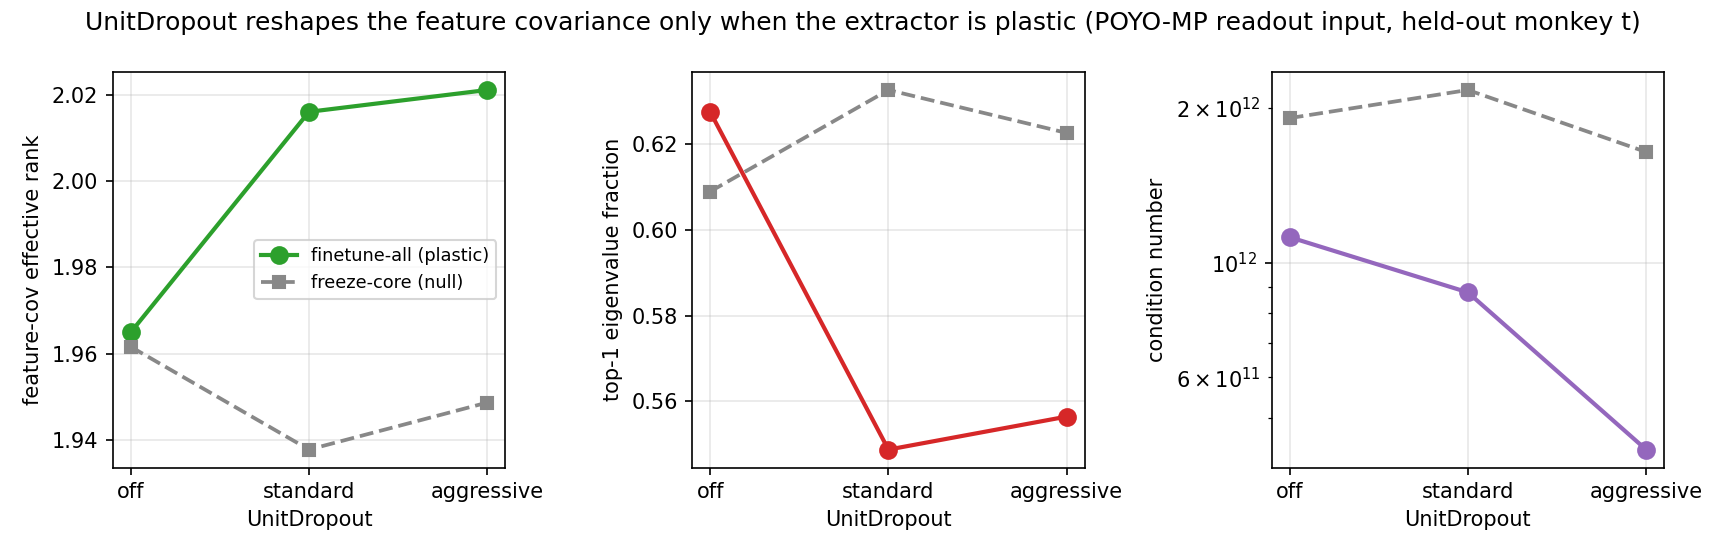
\includegraphics[width=\textwidth]{fig_spectral.png}
\caption{\textbf{UnitDropout reshapes the feature covariance only when the extractor is
plastic.} Finetune-all (solid) spreads the spectrum and cuts the condition number; freeze-core
(dashed) is flat---the null control. The effect is the \citet{lin2024augmentation}
spectral-regularization prediction realized in \poyo's representations.}
\label{fig:spectral}
\end{figure}

\paragraph{The spectral spreading buys generalization---when data is scarce.} A spread spectrum
should help most when the decode is \emph{not} saturated. We close the loop with a
$\{$data fraction$\}\times\{$UnitDropout$\}$ grid (\cref{tab:lowdata}, \cref{fig:lowdata}). At
$10\%$ of the session, augmentation lifts test \rtwo{} from $\ldLoOff$ to $\ldLoAgg$ (monotone,
$+\ldLoGain$), and the off-augmentation model is the most ill-conditioned of the entire grid
($\ldLoCondOff$), which augmentation cuts ${\sim}\ldLoCondDrop\times$ (to $\ldLoCondStd$)---the
conditioning improvement tracks the generalization gain. The gap closes by $25\%$ data and is
flat-to-slightly-negative at full data ($\ldHiOff$ vs.\ $\ldHiAgg$). This is the textbook
data$\times$augmentation interaction, now demonstrated end-to-end on a neural foundation model:
UnitDropout (= the \citeauthor{lin2024augmentation} random-mask augmentation) $\to$
feature-covariance spectral regularization $\to$ a generalization gain, \emph{gated} on both a
plastic feature extractor and data scarcity.

\begin{table}[t]
\centering
\caption{Low-data generalization grid (finetune-all, held-out monkey~t, fixed batch size):
test \rtwo{} vs.\ UnitDropout strength at three training-data fractions. The augmentation
benefit is large under scarcity and vanishes as the decode saturates.}
\label{tab:lowdata}
\poyoLowdataTable
\end{table}

\begin{figure}[t]
\centering
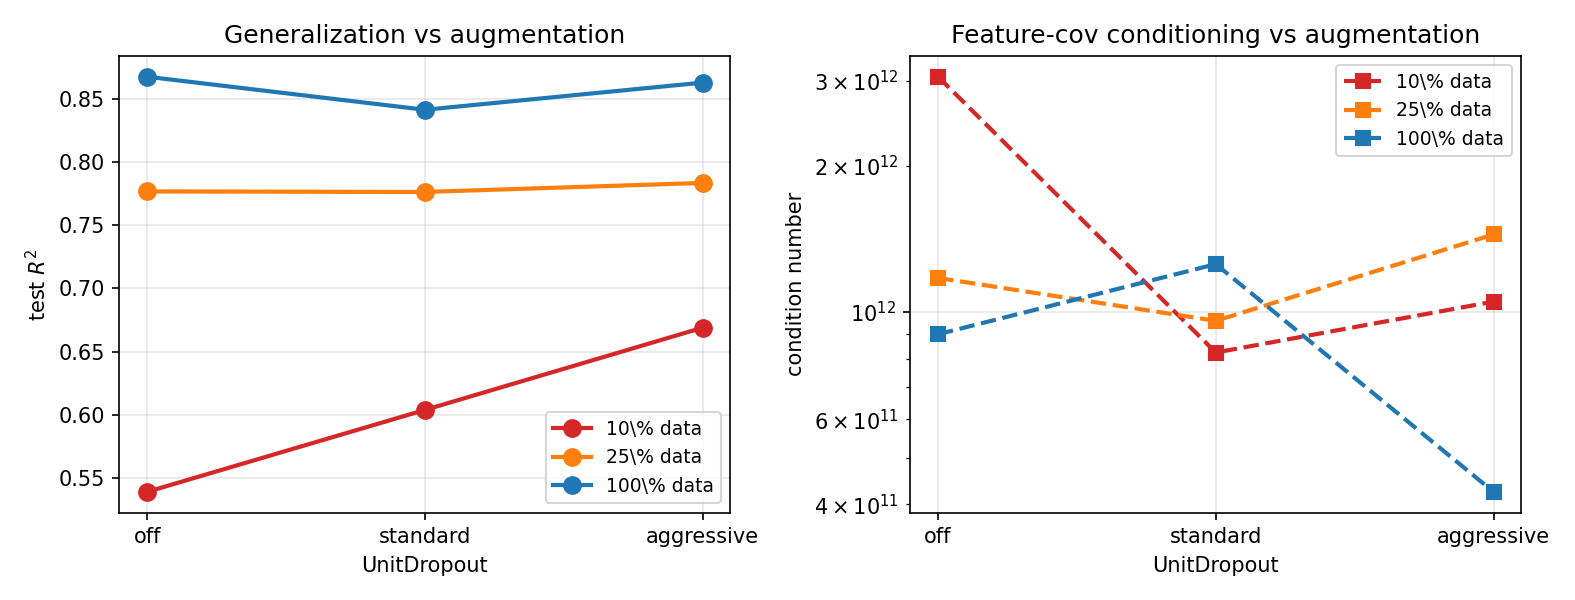
\includegraphics[width=\textwidth]{fig_lowdata.png}
\caption{\textbf{Augmentation buys generalization exactly when data is scarce.} Left:
test \rtwo{} vs.\ UnitDropout, one line per training-data fraction. Right: the feature-covariance
condition number---most ill-conditioned at $10\%$ data with no augmentation, and cut sharply by
UnitDropout, mirroring the generalization gain.}
\label{fig:lowdata}
\end{figure}

\section{Discussion}
\label{sec:discussion}
A faithful reproduction turned \poymp from a target into an instrument. Its representation
transfers strongly across sessions, time, and subjects \emph{within} the motor domain---a few
embedding vectors recover ${\sim}0.9$ \rtwo{} from $10\%$ of a session, hold it for three years,
and port to an unseen animal---and the label-free weight-spectrum quality tracks decode quality
in that regime. The same representation does \emph{not} confer an advantage on cognitive
interval timing, regardless of how the timing target is framed, marking a concrete boundary of
its competence and a case where the spectral$\leftrightarrow$decode correspondence inverts.

The augmentation study connects a clean piece of linear theory \citep{lin2024augmentation} to a
working deep model and pins down its boundary conditions. The predicted spectral regularization
of the feature covariance is real and the generalization payoff is real, but both are gated:
the feature extractor must be plastic, and the decode must not be saturated. The most useful
caveat for practitioners of weight-spectrum diagnostics is the asymmetry we observe---at a
realistic finetuning budget, augmentation's signature is in the representation covariance, not
the weight spectrum---so the feature-covariance and weight-HTSR views answer different
questions and should not be conflated. The main limitations are scope: the cross-subject and
augmentation results use single held-out sessions of one animal, and the weight-spectrum
measurements are at a finetuning (not from-scratch) budget; a multi-animal held-out test set and
a from-scratch augmentation sweep would sharpen the generality of both claims.

\paragraph{Reproducibility.} Every number, table, and figure in this paper is produced from the
raw experiment logs by a single tangle script (\texttt{paper/generate.py}); \texttt{build.sh}
regenerates the manuscript end-to-end. Nothing is hand-transcribed.

\bibliographystyle{iclr2025}
\bibliography{references}

\end{document}
